%We provide some preliminaries used in the following sections of this paper.
\begin{df}
	{\itshape Differentiation Coverage Model}
\end{df}
In the tradition models to evaluate the coverage from the sensing field $S=\{S_1, S_2,..., S_n\}$ toward a point $P$ may lead to several exceptional inconsistency due of these model just depend on distance between sensors in sensing field and the considering point \cite{megerian2002exposure} as follows:\par
All-sensor Field Intensity function
\begin{equation}
\label{equa:01}
E_a(P) = \sum\limits_{i = 1}^N {f({S_i},P)} 
\end{equation}

Closest-sensor Field Intensity function
\begin{equation}
\label{equa:02}
S_{\text{min}}(P) = \underset{s \in S}{\text{argmax}}f(s, P)
\end{equation}
\begin{equation}
\label{equa:03}
E_c(P) = f({S_{\min}(P)},P)
\end{equation}
where $f$ is sensing intensity function that takes two arguments: the first is a sensor and the second is a point.

As a result, we devise a more preferable attenuated model assessing the coverage quality of the sensor network toward a point in the region of interest, the model can later be generalized to evaluate the coverage of the sensor network on a line or a closed region.

Considering a point $P$ lie in the sensing range of a certain omnidirectional or directional sensor. The sensor $S_i$, the penetration object $P$ with radius $R$ and the considered part $P_\phi$ being positioned at $\phi$ and has length $dl$. Call the distance from $S_i$ to $P_\phi$ as $d_i$, the direction of the sensor compared to the pivot direction as $\phi_i$. Because $R$ is usually inconsiderable compared to $d_i$, we can approximately use $\phi_i$ and $d_i$ as constants with variable $\phi$, the model will be now illustrated as followed.

\begin{figure}[!h]
\begin{minipage}{.5\linewidth}
	\centering
	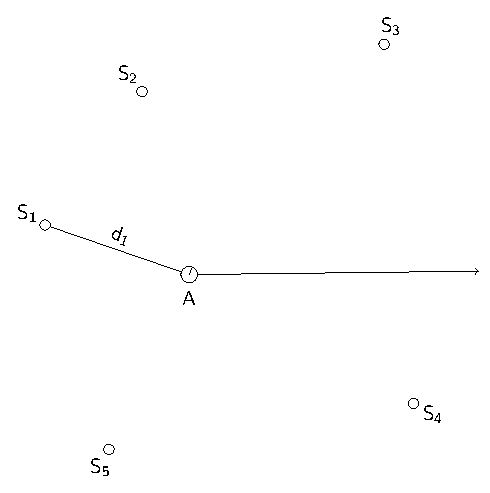
\includegraphics[scale=.75]{groupSensor_Version2.pdf}
\end{minipage}\hfill
\begin{minipage}{.5\linewidth}
	\centering
	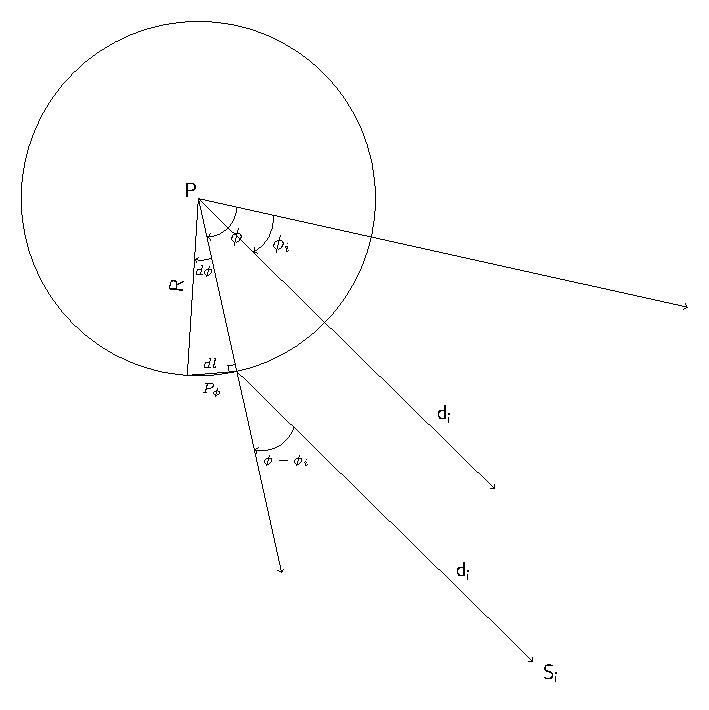
\includegraphics[scale=.6]{exposure.pdf}
\end{minipage}
\end{figure}

Firstly, the coverage value of a sensor to a part is directly affected by the distance between the sensor and the part, and the angle at which the part is viewed by the sensor, this results in the formula:
\begin{equation}
\label{eq1}
\mathsf{max}(\frac{A\cos(\phi - \phi_i)}{Rd_i^\lambda}, 0)dl
\end{equation}


where $\frac{A}{R}$ is a constant coefficient, note that the coverage would fall below 0 if the angle between the direction of the part and the direction of the sensor is larger than $\frac{\pi}{2}$, so we need to set it to 0 in that case. Rewrite $dl = Rd\phi$, we have:
\begin{equation}
\label{eq2}
\mathsf{max}\left\{\frac{A\cos(\phi - \phi_i)}{d_i^\lambda},\ 0\right\}d\phi
\end{equation}

However, it is obviously unnecessary to obtain too much detailed information from the object in the sensing field. This leads to the existence of a constant $E_{\mathsf{max}}$ which corresponds to the maximum necessary coverage on a part with unit length of the circle. To isolate the value from the relative constant $A$, we rewrite it to the Minimum sensing radius $E_{\mathsf{max}} = \frac{A}{d_{\mathsf{min}}^\lambda}$. As a result, our coverage formula could be rewritten as:
\begin{equation}
\label{eq3}
\mathsf{max}\left\{0,\ \mathsf{min}\Big\{\frac{A}{d_{\mathsf{min}}^\lambda}, \frac{Acos(\phi - \phi_1)}{d_i^\lambda}\Big\}\right\}d\phi
\end{equation}

As a result, the coverage on a part $P_\phi$ of several sensors $S_i$, as illustrated above, is the maximum of the coverage on that part of every covered sensor:

\begin{equation}
\label{eq4}
E_\phi(P) = \mathsf{max}\left\{0,\ \mathsf{min}\Big\{\frac{A}{d_{\mathsf{min}}^\lambda},\ \underset{S_i}{\mathsf{max}}\big\{\frac{A\cos(\phi - \phi_i)}{d_i^\lambda}\big\}\Big\}\right\}d\phi
\end{equation}

In short, the coverage on a part of a certain set of sensors is calculated from the largest value of $\displaystyle\frac{Acos(\phi - \phi_1)}{d_i^\lambda}d\phi$ across all sensors, the result then will be a value in the close interval $[0, E_{\mathsf{max}}d\phi]$ that closest to the above computed value. The total coverage on the object is the sum of the coverage on its small parts. Combined with the differentiated form of the formula above, the total coverage would be the integral on all of its parts. As a result, we receive the formula for the total coverage on the object at a certain point in the sensing field:
\begin{equation}
E(P) = \uint\limits_0^{2\pi}{\mathsf{max}\left\{0,\ \mathsf{min}\Big\{\frac{A}{d_{\mathsf{min}}^\lambda}, \ \underset{S_i}{\mathsf{max}}\big(\frac{A\cos(\phi - \phi_i)}{d_i^\lambda}\big)\Big\}\right\}d\phi}
\end{equation}
In conclusion, a new model of coverage is devised which may prove to be exceptionally effective in measuring the coverage efficiency of sensor networks in not only the tradition coverage problem but also in more complex ones such as the problem of $full\hspace{1mm}view$ or multiple view barrier coverage. The new model is proposed with detailed and precise logical progress, successfully adapts the strong points of both the All-Sensor Field Intensity and the Closest-Sensor Field Intensity model \cite{megerian2002exposure}, handling preferably the cooperation of multiple sensors in the network without overrating the repetition of captured information.
%\subsubsection{Coverage of a barrier}	
%\label{bar	rier}

\begin{df}{\itshape Multiple-view barrier}\\
	A multiple-view barrier $B$ is a connected region from the left side to the right side of the monitoring region and satisfies that $B$ is multiple-view covered.
\end{df}
\begin{df}{\itshape Multiple-view barrier coverage}\\
	A region achieves multiple-view barrier coverage if there exists a multiple-view barrier in that region.\par
\end{df}

A multiple-view barrier is a region connecting the left and right side of the sensing field in which all the points are multiple-view covered. Typically, a multiple-view barrier is fairly narrow, and penetration objects usually intersect the barrier only at a small part on their paths. As a result, a proper metric to assess the efficiency of the multiple-view barrier would be the coverage density of it.

With the same set of sensors considered, in the range of coverage of all elements of that set, the coverage function is always continuous. Since a barrier is consisted of several separate parts each of which is multiple-view covered by a common set of sensors, the coverage density of the barrier can be defined as the quotient of the total coverage in the barrier and the area of that area, with the total coverage being formulated as the integral of the sensing intensity function over the barrier region. Call the barrier region $B$ with area $S_B$, the coverage density over $B$, which is $D_B$ can be formulated as
\begin{equation}
\label{eq5}
E(B) = \iint_B{E(x, y)dxdy}.\frac{1}{S_B}
\end{equation}
%Table \ref{tab:01} summarizes all commonly used notations in this paper. Each notation has unique meaning throughout the whole paper.
%\captionsetup[table]{font=large}
%\begin{table}[htb]
%	\centering	
%	\caption{Commonly used notations}
%	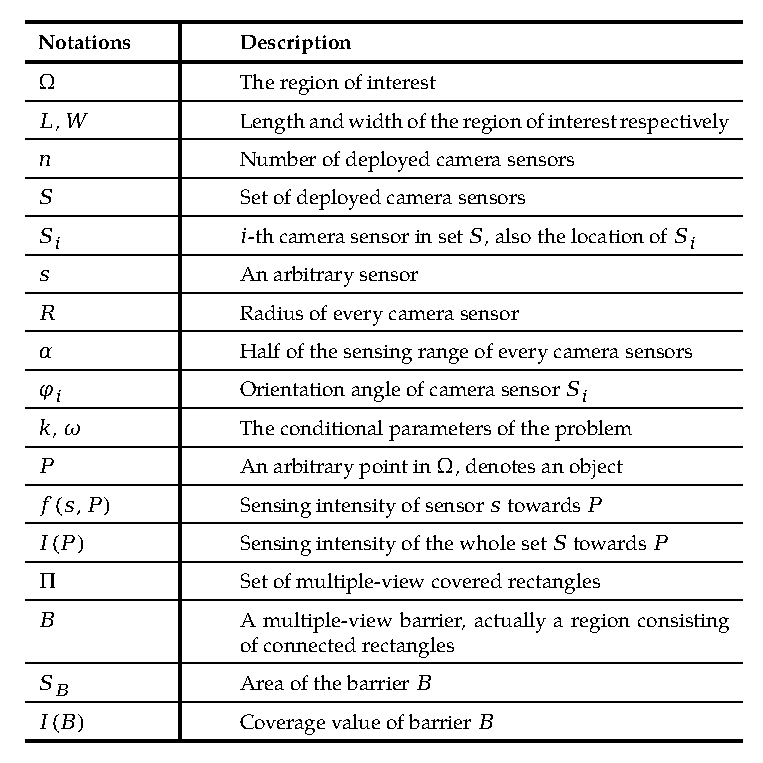
\includegraphics[scale=1.]{Hinhanh/lookup-table}
%	\label{tab:01}
%\end{table}
\renewcommand{\arraystretch}{1.5}
\begin{table}
\centering
\caption{Commonly used notations}
\begin{tabularx}{.8\textwidth}{!{\vline width 1.2pt}Y!{\vline width 1.2pt}Z!{\vline width 1.2pt}}
%	\arrayrulecolor{green}\hline
	\specialrule{1.2pt}{0.pt}{0.pt}
	%%%%%%%%%%%%%%%%%%%%%%%%%%%%%%%%%%%%%%%%%
	{\bfseries Notations} & {\bfseries Description}\\
	\specialrule{1.2pt}{0.pt}{0.pt}
	%%%%%%%%%%%%%%%%%%%%%%%%%%%%%%%%%%%%%%%%%
	$\Omega$ & The region of interest \\
	\specialrule{0.5pt}{0.pt}{0.pt}
	%%%%%%%%%%%%%%%%%%%%%%%%%%%%%%%%%%%%%%%%%
	$L$, $W$ & Length and width of the region of interest respectively \\
	\specialrule{0.5pt}{0.pt}{0.pt}
	%%%%%%%%%%%%%%%%%%%%%%%%%%%%%%%%%%%%%%%%%
	$n$ & Number of deployed camera sensors \\
	\specialrule{0.5pt}{0.pt}{0.pt}
	%%%%%%%%%%%%%%%%%%%%%%%%%%%%%%%%%%%%%%%%%
	$S$ & Set of deployed camera sensors \\
	\specialrule{0.5pt}{0.pt}{0.pt}
	%%%%%%%%%%%%%%%%%%%%%%%%%%%%%%%%%%%%%%%%%
	$S_i$ & $i$-th camera sensor in set $S$, also the location of $S_i$ \\
	\specialrule{0.5pt}{0.pt}{0.pt}
	%%%%%%%%%%%%%%%%%%%%%%%%%%%%%%%%%%%%%%%%%
	$s$ & An arbitrary sensor \\
	\specialrule{0.5pt}{0.pt}{0.pt}
	%%%%%%%%%%%%%%%%%%%%%%%%%%%%%%%%%%%%%%%%%
	$R$ & Radius of every camera sensor \\ 
	\specialrule{0.5pt}{0.pt}{0.pt}
	%%%%%%%%%%%%%%%%%%%%%%%%%%%%%%%%%%%%%%%%%
	$\alpha$ & Half of the sensing range of every camera sensors \\
	\specialrule{0.5pt}{0.pt}{0.pt}
	%%%%%%%%%%%%%%%%%%%%%%%%%%%%%%%%%%%%%%%%%
	$\varphi_i$ & Orientation angle of camera sensor $S_i$ \\
	\specialrule{0.5pt}{0.pt}{0.pt}
	%%%%%%%%%%%%%%%%%%%%%%%%%%%%%%%%%%%%%%%%%
	$k$, $\omega$ & The conditional parameters of the problem \\
	\specialrule{0.5pt}{0.pt}{0.pt}
	%%%%%%%%%%%%%%%%%%%%%%%%%%%%%%%%%%%%%%%%%
	$P$ & An arbitrary point in $\Omega$, denotes an object \\
	\specialrule{0.5pt}{0.pt}{0.pt}
	%%%%%%%%%%%%%%%%%%%%%%%%%%%%%%%%%%%%%%%%%
	$f(s, P)$ & Coverage value of sensor $s$ towards $P$ \\
	\specialrule{0.5pt}{0.pt}{0.pt}
	%%%%%%%%%%%%%%%%%%%%%%%%%%%%%%%%%%%%%%%%%
	$E(P)$ & Coverage value of the whole set $S$ towards $P$ \\
	\specialrule{0.5pt}{0.pt}{0.pt}
	%%%%%%%%%%%%%%%%%%%%%%%%%%%%%%%%%%%%%%%%%
	$\Pi$ & Set of multiple-view covered rectangles \\
	\specialrule{0.5pt}{0.pt}{0.pt}
	%%%%%%%%%%%%%%%%%%%%%%%%%%%%%%%%%%%%%%%%%
	$B$ & A multiple-view barrier, actually a region consisting of connected rectangles \\
	\specialrule{0.5pt}{0.pt}{0.pt}
	%%%%%%%%%%%%%%%%%%%%%%%%%%%%%%%%%%%%%%%%%
	$S_B$ & Area of the barrier $B$ \\
	\specialrule{0.5pt}{0.pt}{0.pt}
	%%%%%%%%%%%%%%%%%%%%%%%%%%%%%%%%%%%%%%%%%
	$E(B)$ & Coverage value of barrier $B$ \\
	\specialrule{1.2pt}{0.pt}{0.pt}
	%%%%%%%%%%%%%%%%%%%%%%%%%%%%%%%%%%%%%%%%%
\end{tabularx}
\end{table}
